\chapter{Sistema Quadrirotore}
Il capitolo è incentrato sulla descrizione del modello matematico del sistema quadricottero con le relative dinamiche, leggi di guida e leggi di controllo possibili da implementare.
\section{Modello matematico}
\todo[inline]{Principi di funzionamento}
Il principio di funzionamento del quadrirotore è relativamente semplice nel suo complesso. Come accennato in precedenza la gestione dell'assetto è ottenuta attraverso l'azionamento differenziale dei rotori, montati su di una struttura rigida \cite{modelquad}.
Nel seguente elenco di manovre di base , viene preso come riferimento la figura \ref{fig:modello_quad}.
\begin{figure}
	\centering
	\begin{subfigure}{0.45\textwidth}
		\centering
		\includegraphics[width=1\textwidth]{SistemaQuadrirotore/Figure/drone_alto}
		\caption{Numerazione rotori}
		\label{fig:modello_quad}
	\end{subfigure}
	\hfill
	\begin{subfigure}{0.45\textwidth}
		\centering
		\includegraphics[width=1\textwidth]{SistemaQuadrirotore/Figure/drone_pitch}
		\caption{Comando per variare il beccheggio}
		\label{fig:modello_quad_pitch}
	\end{subfigure}
	\\
	\begin{subfigure}{0.45\textwidth}
		\centering
		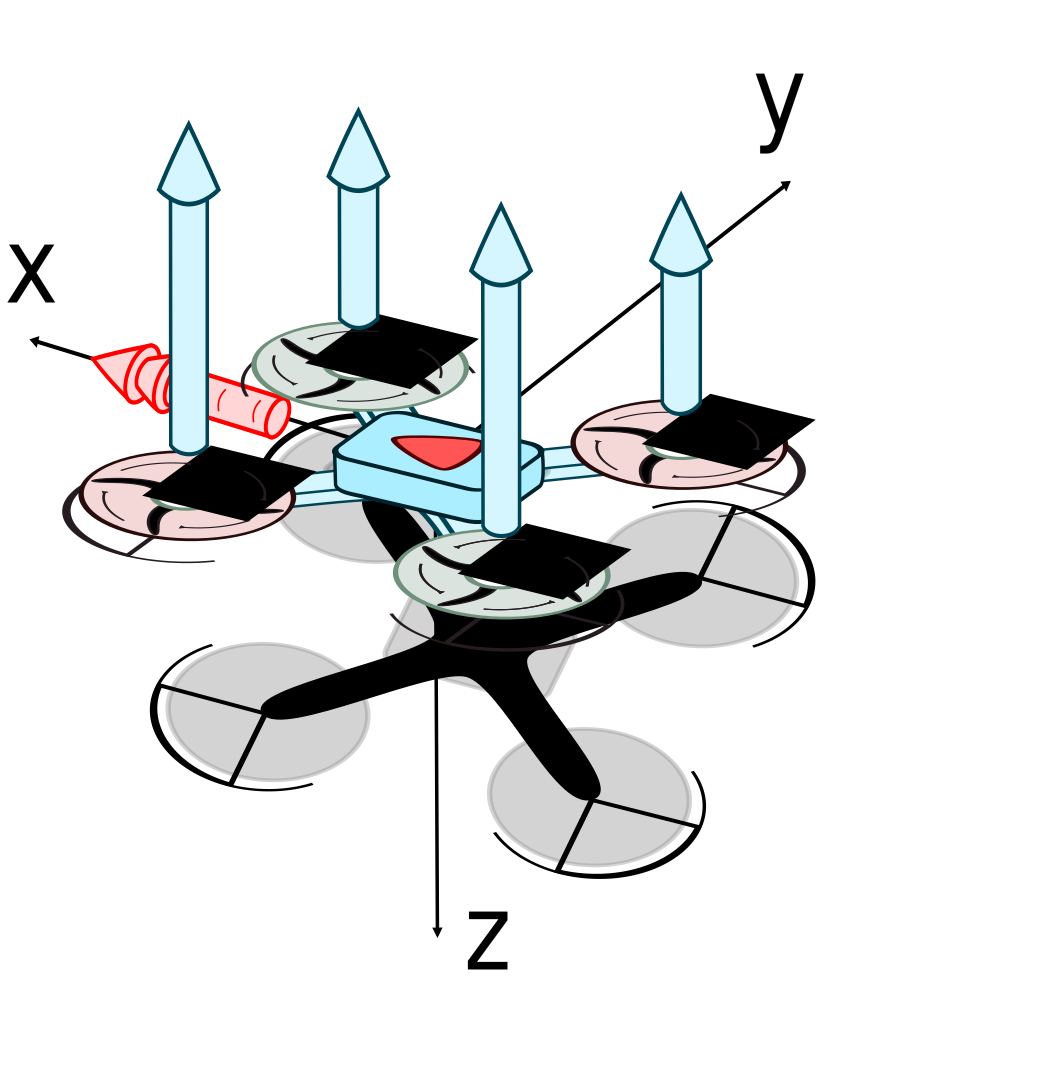
\includegraphics[width=1\textwidth]{SistemaQuadrirotore/Figure/drone_roll}
		\caption{Comando per variare l'angolo di rollio}
		\label{fig:modello_quad_roll}
	\end{subfigure}
	\caption{Schemi semplificati del quadrirotore}
\end{figure}
\begin{itemize}
	\item \textbf{Variazione beccheggio : } una variazione di beccheggio positiva lungo l'asse y del corpo del drone avviene applicanto maggiore forza ai rotori 2 e 3 rispetto ai 1 e 4, come mostrato nella figura \ref{fig:modello_quad_pitch}
	\item \textbf{Variazione rollio :} una variazione di rollio positiva si ottiene ... come mostra la figura \ref{fig:modello_quad_roll}
\end{itemize}
\cite{DesTestCarm}.
\[ 	c(\cdot)=\cos(\cdot)\ ,\  s(\cdot) = \sin(\cdot) \]
\begin{equation}
R=
	\begin{pmatrix}
	c(\psi)c(\theta)-s\phi)s(\psi)s(\theta) & -c(\phi)s(\psi) & c(\psi)s(\theta)+c(\theta)s(\theta)s(\psi) \\ 
	c(\theta) s(\psi)+c(\psi)s(\phi)s(\theta) & c(\phi)c(\psi) & s(\psi)s(\theta)-c(\psi)c(\theta)s(\phi) \\ 
	-c(\phi)s(\theta)	& s(\phi) & c(\phi)c(\theta)
	\end{pmatrix}
\end{equation}
\todo[inline]{il sistema di riferimento}
\todo[inline]{Figura della configurazione del drone
tipo di azionamento base}
\todo[inline]{Definizione degli operatori necessari a descrivere il modello base del drone}
\todo[inline]{Forze e momenti applicati}
\todo[inline]{Breve descrizione alle modifiche fatte al modello per applicazione su gazebo con rimando al capitolo specifico}